\begin{frame}
    \frametitle{Introduction}
    \framesubtitle{UnDeepVO}
    \begin{itemize}
        \item A monocular visual odometry system
    \end{itemize}
\end{frame}

\begin{frame}
    \frametitle{Introduction}
    \framesubtitle{Visual odometry}
    \begin{itemize}
        \item Goal
        \begin{itemize}
            \item Robot localization using only visual information
        \end{itemize}
    \end{itemize}
    \begin{figure}
        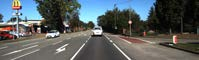
\includegraphics[scale=0.8]{images/road1.png}
        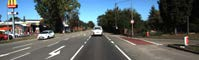
\includegraphics[scale=0.8]{images/road2.png}
        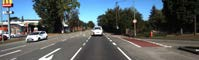
\includegraphics[scale=0.8]{images/road3.png}
        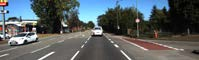
\includegraphics[scale=0.8]{images/road4.png}
    \end{figure}
\end{frame}

\begin{frame}
    \frametitle{Introduction}
    \framesubtitle{Visual odometry}
    \begin{itemize}
        \item Goal
        \begin{itemize}
            \item Use consecutive monocular images to construct a path of robot movement
        \end{itemize}
    \end{itemize}
    \begin{figure}
        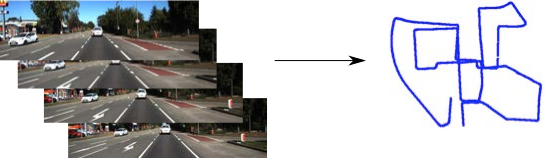
\includegraphics[scale=0.8]{images/vo-objective.png}
    \end{figure}
\end{frame}

\begin{frame}
    \frametitle{Introduction}
    \framesubtitle{UnDeepVO}
    \begin{itemize}
        \item Based on deep learning
        \item Unsupervised
        \begin{itemize}
            \item No need for labeled training data
        \end{itemize}
        \item Pose estimation
        \item Depth estimation
    \end{itemize}
\end{frame}
